% =====================================================================
%  MAT2007 - Introduction to programming, final project report
%  Has the performance gap between F1 cars shrunk?=====================================================================
\documentclass[11pt,a4paper]{article}

\usepackage[utf8]{inputenc}
\usepackage[T1]{fontenc}
\usepackage[margin=2.0cm]{geometry}
\usepackage{graphicx}
\usepackage{amsmath}
\usepackage{booktabs}
\usepackage{siunitx}
\usepackage[hidelinks]{hyperref}
\usepackage{caption}
\captionsetup{font=small}

\title{\vspace{-1.5cm}\bfseries Has the performance gap between Formula~1 cars\\
       closed? A lap-time analysis of 1996--2024}
\author{Matas Joffe (ID: 6429832)}   
\date{\today}

\begin{document}
\maketitle
\vspace{-0.9cm}

% =====================================================================
\section{Introduction}
% =====================================================================
Formula~1 is a sport in which the machine matters at least as much as the
driver, and for most of its history the grid has been sharply divided between a
few works teams and a tail of entries several seconds per lap slower. Since the
1990s the governing body has introduced restrictive technical regulations,
standardised components and, from 2021, a budget cap, all with the stated aim of
closing that gap. This report asks whether the gap has in fact closed, and if
so, \emph{why}: have
the cars genuinely converged, or has the slow tail of the grid simply stopped
entering? The two explanations predict different things and can be separated in
the data. The analysis covers 1996--2024, the period for which individual lap
times exist.

% =====================================================================
\section{Data sample}
% =====================================================================
We use the \emph{Formula~1 World Championship} dataset, a public release of the
Ergast motor-racing database hosted on Kaggle~\cite{dataset}. Four files are
used: \texttt{lap\_times.csv} (every individual lap, in milliseconds),
\texttt{results.csv} (which driver drove which car), \texttt{races.csv} and
\texttt{constructors.csv}. The championship goes back to 1950, but lap-by-lap
timing begins only in 1996, which sets the start of the sample.

Three cleaning steps were applied: lap times outside
\SIrange{30}{300}{\second} were discarded as timing errors or cars limping to the
pits; opening laps were removed, as they start from a standstill; and a
constructor was counted in a race only if at least 20~timed laps were recorded
for it, so that a car which crashed early cannot contribute a meaningless
``best lap''. After cleaning, \textbf{542 races} entered the analysis.

% =====================================================================
\section{Analysis method}
% =====================================================================
For each race and each constructor we take the single fastest lap set by either
of its cars. The minimum is used rather than the mean because a car's best lap
is close to its true potential, whereas its average lap is contaminated by
traffic, fuel load and pit stops. Two quantities are then formed per race:
%
\begin{equation}
  G_{\text{full}} = 100\,\frac{t_{\text{slowest}} - t_{\text{fastest}}}{t_{\text{fastest}}},
  \qquad
  G_{\text{trim}} = 100\,\frac{t_{\text{2nd slowest}} - t_{\text{fastest}}}{t_{\text{fastest}}}\quad [\%].
\end{equation}
%
$G_{\text{full}}$ measures how wide the grid is; $G_{\text{trim}}$ ignores the
single slowest constructor and so measures how close the rest of the field is.
If the two behave alike, the cars have converged; if only $G_{\text{full}}$
falls, the change is in who enters, not in the machinery. Percentages are used
so that circuits of different lap lengths can be compared.

Races are aggregated per season using the median, which is insensitive to the
few wet or safety-car-dominated events that would distort a mean; the
uncertainty on the median is $1.253\,\sigma/\sqrt{N}$. Season medians are then
averaged within eras by inverse-variance weighting. The analysis uses
\texttt{pandas} and \texttt{numpy}.

% =====================================================================
\section{Results and discussion}
% =====================================================================
Figure~\ref{fig:trend} shows both quantities per season. The field spread is
clearly \emph{not} a smooth function of time: a straight-line fit over the whole
period returns a slope of $-0.024 \pm 0.026$ percentage points per year, only
$0.9\sigma$ from zero, with $\chi^2/\mathrm{ndf} = 14.4$. A linear trend is
simply the wrong model.

\begin{figure}[htbp]
  \centering
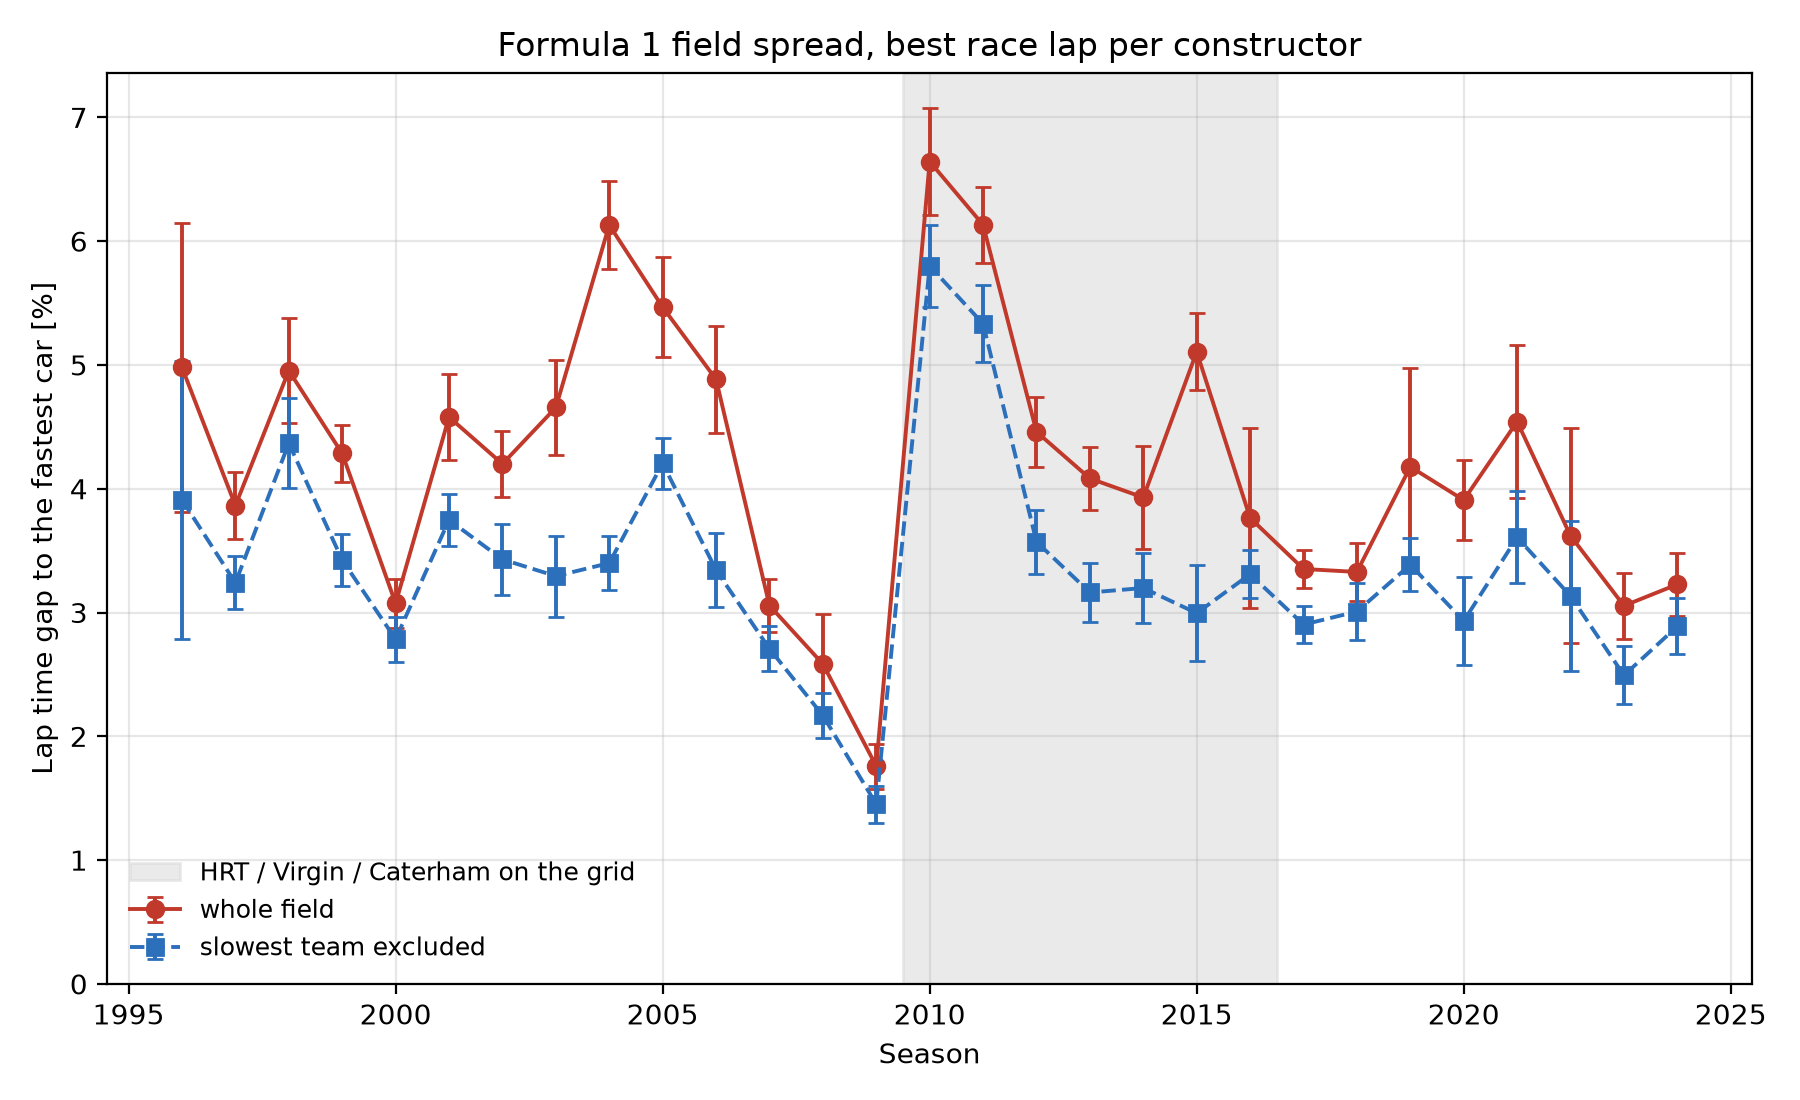
\includegraphics[width=0.56\textwidth]{gap_trend.png}
  \caption{Season-median lap-time gap to the fastest car, for the whole field
  (red) and with the single slowest constructor excluded (blue). The shaded band
  marks the seasons in which HRT, Virgin/Marussia and Lotus/Caterham were on the
  grid.}
  \label{fig:trend}
\end{figure}

The reason is visible in the figure. The gap peaks at
$4.88 \pm 0.13\,\%$ during 2010--2016, the years in which three new teams
entered the championship far off the pace, and this excursion cancels the
decline on either side of it. Within eras the gap does fall: $-0.154 \pm 0.071$
percentage points per year over 1996--2009 and $-0.098 \pm 0.037$ over
2012--2024.

Comparing like with like, by setting the new-team years aside, gives the
headline result (Table~\ref{tab:eras}). For the whole field the gap falls from
$4.00 \pm 0.08\,\%$ to $3.39 \pm 0.10\,\%$, a reduction of
$0.61 \pm 0.13\,\%$, or $4.7\sigma$. Excluding the single slowest car, however,
the same comparison gives only $0.22 \pm 0.11\,\%$ ($2.1\sigma$). The bulk of
the narrowing is therefore carried by the slowest constructor alone: the tail of
the grid has disappeared, while the remaining cars have converged only
marginally. The two differences are correlated, being measured on the same
races, so their gap indicates size rather than an independent significance.

\begin{table}[htbp]
  \centering\small
  \begin{tabular}{lccc}
    \toprule
    & 1996--2008 & 2010--2016 & 2017--2024 \\
    \midrule
    Whole field [\%]            & $4.00 \pm 0.08$ & $4.88 \pm 0.13$ & $3.39 \pm 0.10$ \\
    Slowest team excluded [\%]  & $3.20 \pm 0.06$ & $3.74 \pm 0.10$ & $2.98 \pm 0.08$ \\
    \bottomrule
  \end{tabular}
  \caption{Inverse-variance weighted mean of the season medians in each era.}
  \label{tab:eras}
\end{table}

Two caveats remain. The metric uses race laps, where a slow car in clear air can
out-pace a fast car in traffic; qualifying times would be cleaner but do not
cover the full period. And the number of constructors varies between 10 and 13,
which matters because a maximum over more teams is larger on average -- part of
why $G_{\text{trim}}$ is the more stable quantity.

\paragraph{Conclusion.} The gap between the fastest and slowest Formula~1 car
has not shrunk steadily since 1996; it is governed by whether backmarker teams
are present, and widened to $4.88 \pm 0.13\,\%$ when three of them joined in
2010. Comparing grids of similar composition, the field is
$0.61 \pm 0.13\,\%$ tighter in 2017--2024 than in 1996--2008 ($4.7\sigma$), but
only $0.22 \pm 0.11\,\%$ of that survives when the slowest car is removed. Most
of the convergence is the disappearance of the slow tail rather than the cars
themselves growing alike.

% =====================================================================
\small
\begin{thebibliography}{9}\itemsep0pt
\bibitem{dataset}
  V.~Rao, \emph{Formula 1 World Championship (1950--2024)}, Kaggle, derived from
  the Ergast Developer API,
  \url{https://www.kaggle.com/datasets/rohanrao/formula-1-world-championship-1950-2020}
  (accessed \today).
\end{thebibliography}

\end{document}